\documentclass[tikz,border=8pt]{standalone}
% Shared look for every TikZ diagram. Load with \input{../../tools/tikz-style.tex}
\usepackage[sfdefault]{roboto}
\usetikzlibrary{arrows.meta, positioning, shapes.geometric, calc, fit, backgrounds}
\definecolor{cblue}{HTML}{4C78A8}
\definecolor{corange}{HTML}{F58518}
\definecolor{cgreen}{HTML}{54A24B}
\definecolor{cred}{HTML}{E45756}
\definecolor{cpurple}{HTML}{B279A2}
\definecolor{cgrey}{HTML}{6B6B6B}
\tikzset{
  every picture/.style={font=\sffamily, line width=1.2pt},
  box/.style={draw=#1, fill=#1!12, rounded corners=4pt, align=center, inner sep=7pt, minimum height=1.1cm},
  box/.default=cgrey,
  arrow/.style={-{Stealth[length=3mm]}, draw=cgrey, line width=1.4pt},
  title/.style={font=\sffamily\bfseries\Large},
  note/.style={font=\sffamily\small, text=cgrey, align=center},
}
\AtBeginDocument{\hyphenpenalty=10000 \exhyphenpenalty=10000}

% The heading loop cut open. Heading command -> comparison -> PD controller C(s) = Kp + Kd s -> torque -> heading plant
% G(s) = 1/(0.1 s^2) -> heading -> delay e^{-s tau} -> back to the comparison with a minus sign. Cut at the torque:
% a signal injected at A goes once round and comes out at B multiplied by -L(s), L(s) = C(s) G(s) e^{-s tau}.
\begin{document}
\begin{tikzpicture}[every node/.append style={font=\large}]
  \node[circle, draw=cgrey, fill=white, minimum size=0.9cm, inner sep=0pt] (cmp) at (0,0) {};
  \node[font=\Large] at ($(cmp.north west)+(-0.2,0.2)$) {$+$};
  \node[font=\Large] at ($(cmp.south east)+(0.25,-0.25)$) {$-$};
  \node[box=cgreen, text width=3.3cm] (C) at (3.6,0) {\textbf{controller}\\[3pt] $C(s) = K_p + K_d\,s$\\[2pt]
     \small\textcolor{cgrey}{$0.4 + 0.08\,s$ (N\,m/rad)}};
  \node[box=cblue, text width=3.3cm] (G) at (12.2,0) {\textbf{heading plant}\\[3pt] $G(s) = \dfrac{1}{0.1\,s^2}$\\[2pt]
     \small\textcolor{cgrey}{torque in, heading out}};
  \node[box=corange, text width=3.3cm] (D) at (8.0,-3.4) {\textbf{delay}\\[3pt] $e^{-sT_d}$\\[2pt]
     \small\textcolor{cgrey}{heading arrives $T_d$ s late}};
  % the cut
  \coordinate (B) at (6.6,0);
  \coordinate (A) at (8.4,0);
  \draw[arrow] (-2.4,0) -- node[below] {command} (cmp.west);
  \draw[arrow] (cmp.east) -- node[above] {error} (C.west);
  \draw[arrow, draw=cred] (C.east) -- (B);
  \draw[arrow, draw=cred] (A) -- node[above, text=black] {torque} (G.west);
  \draw[cred, line width=1.6pt] ($(B)+(0.5,0.55)$) -- ($(B)+(0.5,-0.55)$);
  \draw[cred, line width=1.6pt] ($(A)+(-0.5,0.55)$) -- ($(A)+(-0.5,-0.55)$);
  \node[text=cred, font=\large\bfseries] at ($(B)+(0,0.85)$) {B};
  \node[text=cred, font=\large\bfseries] at ($(A)+(0,0.85)$) {A};
  \node[note, text=cred, font=\normalsize] at (7.5,1.75) {cut here: a signal put in at A\\comes out at B};
  \draw[arrow] (G.east) -- node[above] {heading $\theta$} (16.2,0);
  \draw[arrow] (15.2,0) |- (D.east);
  \draw[arrow] (D.west) -| (cmp.south);
  \node[note, font=\normalsize, anchor=north] at (8.0,-4.7) {once round, A to B: $C(s)\,G(s)\,e^{-sT_d}$ and the minus sign,\\
     so B $=-L(s)\times$ A with the loop transfer function $L(s) = C(s)\,G(s)\,e^{-sT_d}$};
  \node[note, font=\small, anchor=north] at (3.6,-1.3) {the derivative acts on the measured\\heading only; round the loop it still\\multiplies by $K_p + K_d\,s$};
\end{tikzpicture}
\end{document}
